\chapter{Properties}
\label{Properties}

\paragraph{}
In this chapter we discuss the implications of what we have seen in the previous chapter. The implications of Property~\ref{intersection-patterns} on the possible permutation representation graphs. We start with a direct consequence of the definition of a permutation representation graph.

\begin{proposition}
  \label{fixed-only-1}
  In a permutation representation graph, two edges with the same index cannot be adjacent.
\end{proposition}

\begin{proof}
  Here is one graph of the situation

  \begin{figure}[H]
    \begin{center}
      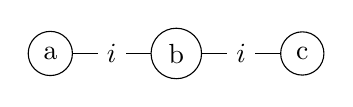
\begin{tikzpicture}[scale=.8]

        \begin{scope}[every node/.style={circle,draw}]
          \node (1)  at (0,0)  {a};
          \node (2)  at (2,0)  {b};
          \node (3)  at (4,0)  {c};
        \end{scope}

        \begin{scope}[every node/.style={fill=white}]

          \begin{scope}[every edge/.style={draw}]
            \path (1)  edge node {$i$} (2);
            \path (2)  edge node {$i$} (3);
          \end{scope}
        \end{scope}

      \end{tikzpicture}
      \caption{}
    \end{center}
  \end{figure}

  \paragraph{}
  If a such graph exist then, by definition of a permutation representation graph, because there is an edge labeled with $i$ between $a$ and $b$, then this mean that $a \rho_i = b$ and $b \rho_i = a$. But there is also an edge labeled with $i$ between $b$ and $c$, thus $b \rho_i = c$ and $c \rho_i = b$. There is a contradiction because $a = b \rho_i = c$ but $a \neq c$. Thus this graph is impossible.
\end{proof}

\paragraph{}
First we define three patterns that are used in the construction of the permutation representation graphs.

\section{Definitions}
\begin{definition}[Alternating square]
  \index{alternating square}
  An alternating edge is a set of 4 vertices and 4 edges that form the following graph:

  \begin{figure}[H]
    \begin{center}
      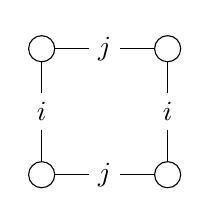
\begin{tikzpicture}[scale=.8]

        \begin{scope}[every node/.style={circle,draw}]
          \node (1)  at (0,2)  {};
          \node (2)  at (0,0)  {};
          \node (3)  at (2,2)  {};
          \node (4)  at (2,0)  {};
        \end{scope}

        \begin{scope}[every node/.style={fill=white}]

          \begin{scope}[every edge/.style={draw}]
            \path (1)  edge node {$i$} (2);
            \path (3)  edge node {$i$} (4);
            \path (1)  edge node {$j$} (3);
            \path (2)  edge node {$j$} (4);
          \end{scope}
        \end{scope}

      \end{tikzpicture}
      \caption{}
    \end{center}
  \end{figure}

  \paragraph{}
  Additional edges can be present on the permutation representation graph, if there exists 4 edges and 4 vertices that form the previous graph, then there is an alternating square.

  \paragraph{}
  This alternating square is denoted $[\rho_i, \rho_j]$
\end{definition}

\begin{definition}[Multiple edge]
  \index{multiple edge}
  \index{double edge}

  A \textit{multiple edge} is a pair of vertices and a set of at least two edges linking those vertices. The number of edges is called the multiplicity of the multiple edge. If the multiplicity is exactly two, it is called a \textit{double edge}.

  \begin{figure}[H]
    \begin{center}
      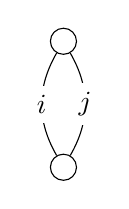
\begin{tikzpicture}[scale=.8]

        \begin{scope}[every node/.style={circle,draw}]
          \node (1)  at (0,2)  {};
          \node (2)  at (0,0)  {};
        \end{scope}

        \begin{scope}[every node/.style={fill=white}]

          \begin{scope}[every edge/.style={draw}]
            \path (1)  edge[bend right=30] node {$i$} (2);
            \path (1)  edge[bend left=30] node {$j$} (2);
          \end{scope}
        \end{scope}

      \end{tikzpicture}
      \caption{}
    \end{center}
  \end{figure}

  \paragraph{}
  A double edge is denoted $(\rho_i, \rho_j)$.
\end{definition}

\begin{definition}[Single edge]
  A single edge is a pair of vertices and an edge such that both vertices are not in the same alternating square or in the same multiple edge.
\end{definition}

\paragraph{}
Now we continue with the implications on the permutation representation graphs.

\section{Single edge}

\begin{definition}
  An edge (simple or multiple) is called adjacent to another pattern if they share exactly one vertex.
\end{definition}

\begin{definition}
  A sequence of single edges will be called a chain.
\end{definition}

\begin{proposition}
  \label{chain-consecutive}
  In a chain, the indices of two adjacent edges must be consecutive.
\end{proposition}

\begin{proof}
  currently the situation is this graph

  \begin{figure}[H]
    \begin{center}
      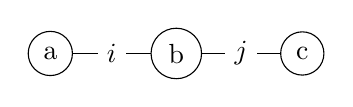
\begin{tikzpicture}[scale=.8]

        \begin{scope}[every node/.style={circle,draw}]
          \node (1)  at (0,0)  {a};
          \node (2)  at (2,0)  {b};
          \node (3)  at (4,0)  {c};
        \end{scope}

        \begin{scope}[every node/.style={fill=white}]

          \begin{scope}[every edge/.style={draw}]
            \path (1)  edge node {$i$} (2);
            \path (2)  edge node {$j$} (3);
          \end{scope}
        \end{scope}

      \end{tikzpicture}
      \caption{}
    \end{center}
  \end{figure}

  \paragraph{}
  If $i$ and $j$ are not consecutive, the graph obtained from the permutation representation graph where only the $\rho_i$ and $\rho_j$ edges are kept must only form the patterns displayed in Property~\ref{intersection-patterns}.

  \paragraph{}
  The pattern the graph cannot form fixed points, distinct single edges or a double edge. Thus the only remaining pattern of Property~\ref{intersection-patterns} is the alternating square. But if those two edges are part of an alternating square, there are no more single edges and thus they does not form a chain which is a contradiction.

  \paragraph{}
  Thus in a chain, the indices must be consecutive.
\end{proof}

\section{Multiple edge}

\begin{proposition}
  A multiple edge with multiplicity three or more cannot be connected to a single edge\footnote{Unused}.
\end{proposition}

\begin{proof}
\end{proof}

\begin{proposition}
  A double edge cannot be adjacent to either an alternating square or another double edge\footnote{Unused}.
\end{proposition}

\begin{definition}
  A double edge is included into an alternating square if both vertices of the double edge are vertices of the alternating square.
\end{definition}

\begin{proposition}
  \label{adjacent-double}
  A double edge $(\rho_i, \rho_j)$ can only be adjacent to a simple edge if the difference between the indices of its edges is exactly 2. In this case the index of the single edge must be in the middle of the indices of the double edge i.e. if the index of the simple edge is $k$ then $|i-k| = 1$ and $|j-k| = 1$.
\end{proposition}

\begin{corollary}
  \label{continue-double-edge}
  Let $(\rho_i, \rho_j)$ be a double edge. If $|i - j| \neq 2$ then the double edge must be included into an alternating square. Furthermore the alternating square must be  $[\rho_{i-1}, \rho_j]$, $[\rho_{i+1}, \rho_j]$, $[\rho_i, \rho_{j-1}]$ or $[\rho_i, \rho_{j+1}]$.
\end{corollary}

\begin{proposition}
  \label{continue-triple-edge}
  A triple edge or a quadruple edge can only be connected to an alternating square.
\end{proposition}

\section{Alternating square}

\begin{notation}
  An alternating square between involutions $\rho_i$ and $\rho_j$ will be denoted $[\rho_i, \rho_j]$.
\end{notation}

\begin{proposition}
  \label{square-connection}
  Given an alternating square $[\rho_i, \rho_j]$ a single edge can be adjacent to this square only if $|i - j| = 2$. In this case the index of the single edge will be in in the middle of the two indices i.e. if the index of the edge is $k$ then $|i-k| = 1$ and $|j-k| = 1$.
\end{proposition}

\begin{definition}
  Two alternating square are adjacent if they share two vertices.
\end{definition}

\begin{proposition}
  \label{adjacent-squares}
  Given an alternating square $[\rho_i, \rho_j]$ the only possible adjacent alternating square are $[\rho_{i-1}, \rho_j], [\rho_{i+1}, \rho_j], [\rho_i, \rho_{j-1}]$ or $[\rho_i, \rho_{j+1}]$.
\end{proposition}

\begin{corollary}
  \label{continue-alternating-square}
  If the difference between the indices of an alternating square is not 2, then it can only be adjacent to another alternating square.
\end{corollary}

\begin{corollary}
  If two alternating square are adjacent, then the difference between the difference of the indices of the square is exactly 1.
\end{corollary}

\paragraph{}
Due to the fact that some alternating square must be adjacent to other one, we will study the sequence of alternating squares.

\begin{corollary}
  \label{parity-sequence-squares}
  If an alternating square in a sequence can be connected to a single edge then the number of square in the sequence before the next square with this property in sequence is odd.
\end{corollary}

\paragraph{}
There are a number a special patterns that achieve a given goal. Those pattern are unique.

\begin{proposition}
  \label{rotation-pattern}
  The single rotation pattern is the following

  \begin{figure}[H]
    \begin{center}
      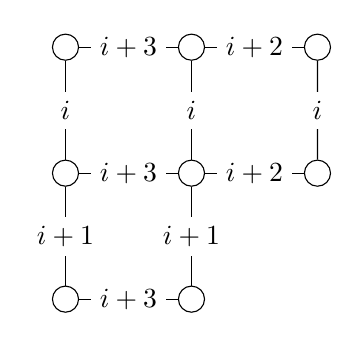
\begin{tikzpicture}[scale=.8]

        \begin{scope}[every node/.style={circle,draw}]
          \node (1)  at (0,2)  {};
          \node (2)  at (0,0)  {};
          \node (3)  at (0,-2) {};
          \node (4)  at (2,2)  {};
          \node (5)  at (2,0)  {};
          \node (6)  at (2,-2) {};
          \node (7)  at (4,2)  {};
          \node (8)  at (4,0)  {};
        \end{scope}

        \begin{scope}[every node/.style={fill=white}]

          \begin{scope}[every edge/.style={draw}]
            \path (2)  edge node {$i+1$} (3);
            \path (5)  edge node {$i+1$} (6);
            \path (1)  edge node {$i$} (2);
            \path (4)  edge node {$i$} (5);
            \path (7)  edge node {$i$} (8);
            \path (1)  edge node {$i+3$} (4);
            \path (2)  edge node {$i+3$} (5);
            \path (3)  edge node {$i+3$} (6);
            \path (4)  edge node {$i+2$} (7);
            \path (5)  edge node {$i+2$} (8);
          \end{scope}
        \end{scope}

      \end{tikzpicture}
      \caption{}
    \end{center}
  \end{figure}

\end{proposition}

\begin{proposition}
  \label{linear-pattern}
  The single linear pattern that allow to change the vertical index of the sequence is the following:

  \begin{figure}[H]
    \begin{center}
      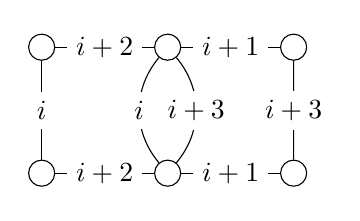
\begin{tikzpicture}[scale=.8]

        \begin{scope}[every node/.style={circle,draw}]
          \node (1)  at (0,2)  {};
          \node (2)  at (0,0)  {};
          \node (3)  at (2,2)  {};
          \node (4)  at (2,0)  {};
          \node (5)  at (4,2)  {};
          \node (6)  at (4,0)  {};
        \end{scope}

        \begin{scope}[every node/.style={fill=white}]

          \begin{scope}[every edge/.style={draw}]
            \path (1)  edge node {$i$} (2);
            \path (3)  edge[bend right=40] node {$i$} (4);
            \path (1)  edge node {$i+2$} (3);
            \path (2)  edge node {$i+2$} (4);
            \path (3)  edge node {$i+1$} (5);
            \path (4)  edge node {$i+1$} (6);
            \path (3)  edge[bend left=40] node {$i+3$} (4);
            \path (5)  edge node {$i+3$} (6);

          \end{scope}
        \end{scope}

      \end{tikzpicture}
      \caption{}
    \end{center}
  \end{figure}

\end{proposition}

\begin{corollary}
  \label{sequence-connection}
  A sequence that cannot be extended can only be adjacent to a single edge.
\end{corollary}

\section{General properties}

\begin{proposition}
  \label{patterns-adding}
  When adding edge of an involution $\rho_i$ to an existing permutation representation graph, for each $\rho_j$ that must commute with $\rho_i$, the following pattern are possible:
  \begin{enumerate}
    \item Form an alternating square $[\rho_i, \rho_j]$
    \item Double an existing $\rho_j$ edge and form a double edge $(\rho_i, \rho_j)$
    \item Link two points fixed by $\rho_j$.
  \end{enumerate}
\end{proposition}
